\documentclass[8pt]{beamer}

\usetheme{metropolis}

\usepackage{varwidth}
\usepackage{xcolor}

\date{19.01.23}
\title{Introduction to Machine Learning}
\subtitle{Image recognition in Python and Tensorflow}
\author{Esten H. Leonardsen and Martin Hovin}

\titlegraphic{
	\centering
}

\begin{document}
	\begin{frame}
		\maketitle
	\end{frame}

	\begin{frame}{Introduction} % Speakers
		\centering
		\vfill
		\begin{tikzpicture}
			\node[] (esten) at (0, 0) {
				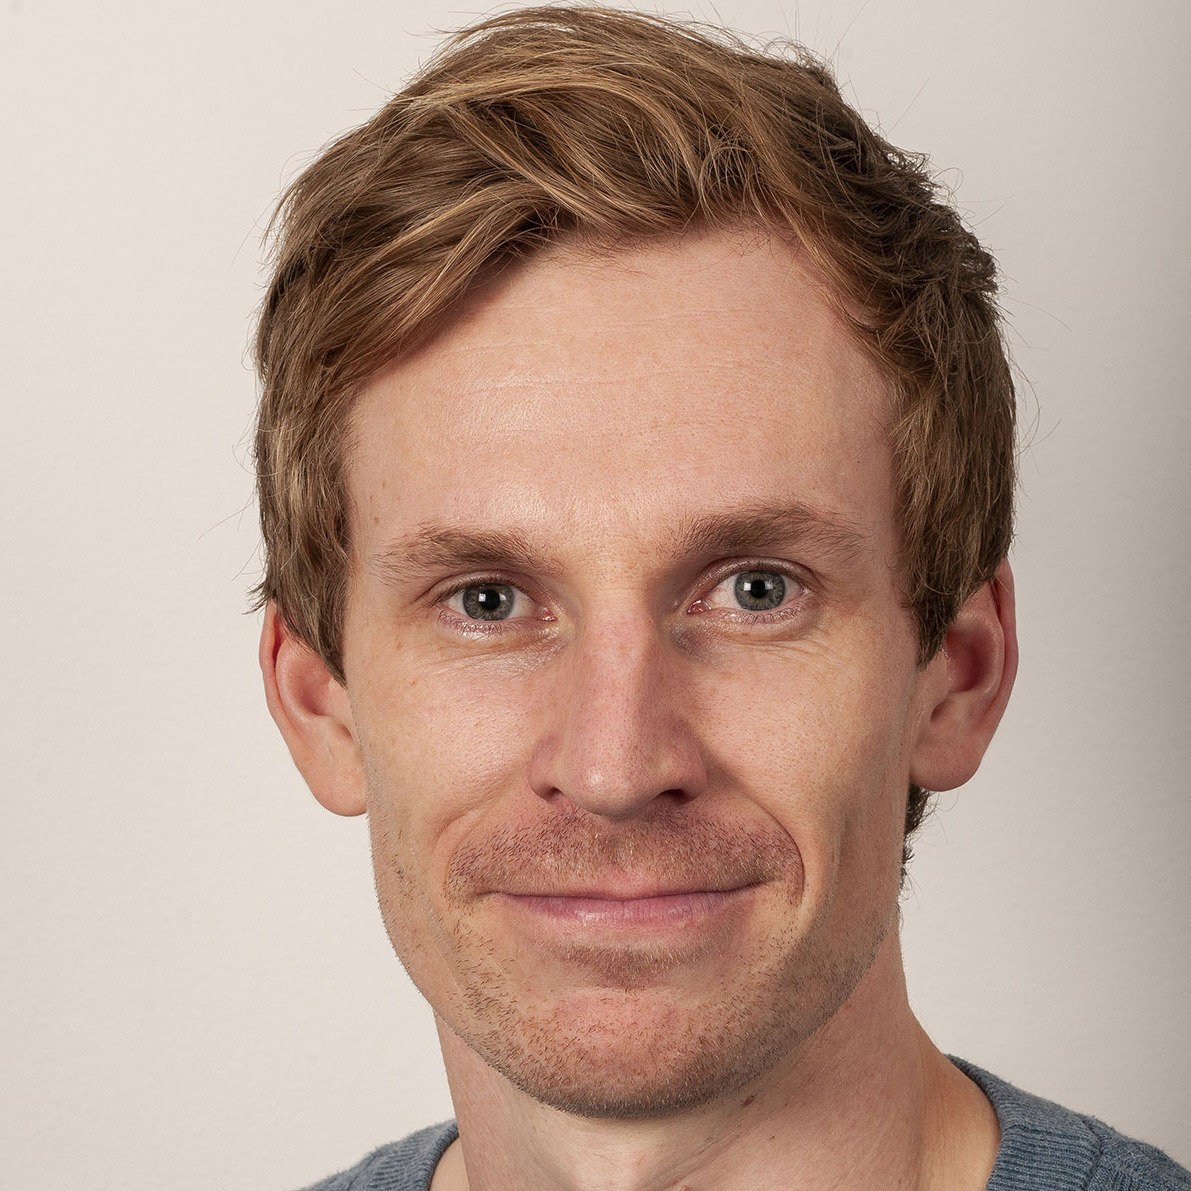
\includegraphics[width=2cm]{data/esten.jpg}
			};
			\node[] (martin) at (0, -3) {
				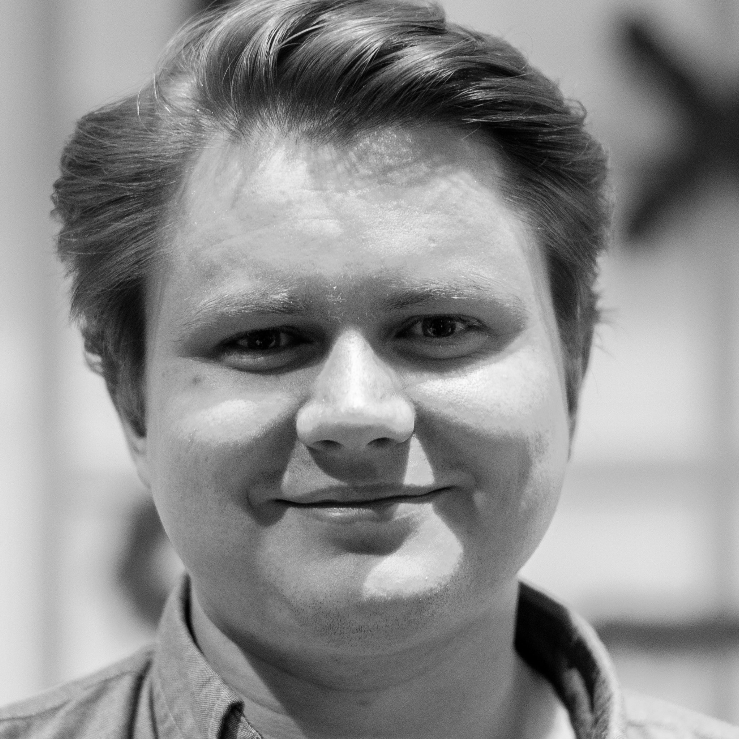
\includegraphics[width=2cm]{data/martin.png}
			};
			\node[align=left, anchor=west] at (esten.east) {
				\textbf{Esten H. Leonardsen}\\
				(UiO and Biometrical AS)\\
				\underline{Interests:}\\
				- Talking about esoteric theory\\
				- Making deep learning tutorials
			};
			\node[align=left, anchor=west] at (martin.east) {
				\textbf{Martin Hovin}\\
				(Biometrical AS)\\
				\underline{Interests:}\\
				- Installing tensorflow\\
				- Debugging Estens code
			};
		\end{tikzpicture}
		\vfill
	\end{frame}

	\begin{frame}{Introduction} % Learning goals
		\vfill
		Theory session:
		\begin{itemize}
			\item What is a statistical learning model?
			\item What is a loss function?
			\item How do we train a statistical learning model?
			\item How does a (deep) neural network work?
			\item What operations does a convolutional neural network use?
			\item What is transfer learning?
			\item What is overfitting?
			\item How do we combat it?
		\end{itemize}
		Practical session:
		\begin{enumerate}
			\item Set up a Python-environment containing Tensorflow
			\item Use a pretrained convolutional neural network to predict
			\item Fit a flower classifier using transfer learning
			\item Improve the flower classifier
		\end{enumerate}
		\vfill
	\end{frame}

	\begin{frame}{Introduction} % Motivation: Brain classification
	\end{frame}

	\begin{frame}{Introduction} % Motivation: Biometrical
	\end{frame}

	\begin{frame}{Introduction} % Motivation: Gjensidige
	\end{frame}

	\begin{frame}{Introduction} % Motivation: Segmentation
	\end{frame}

	\begin{frame}{Introduction} % Motivation: Imagen
		\centering
		\vfill
		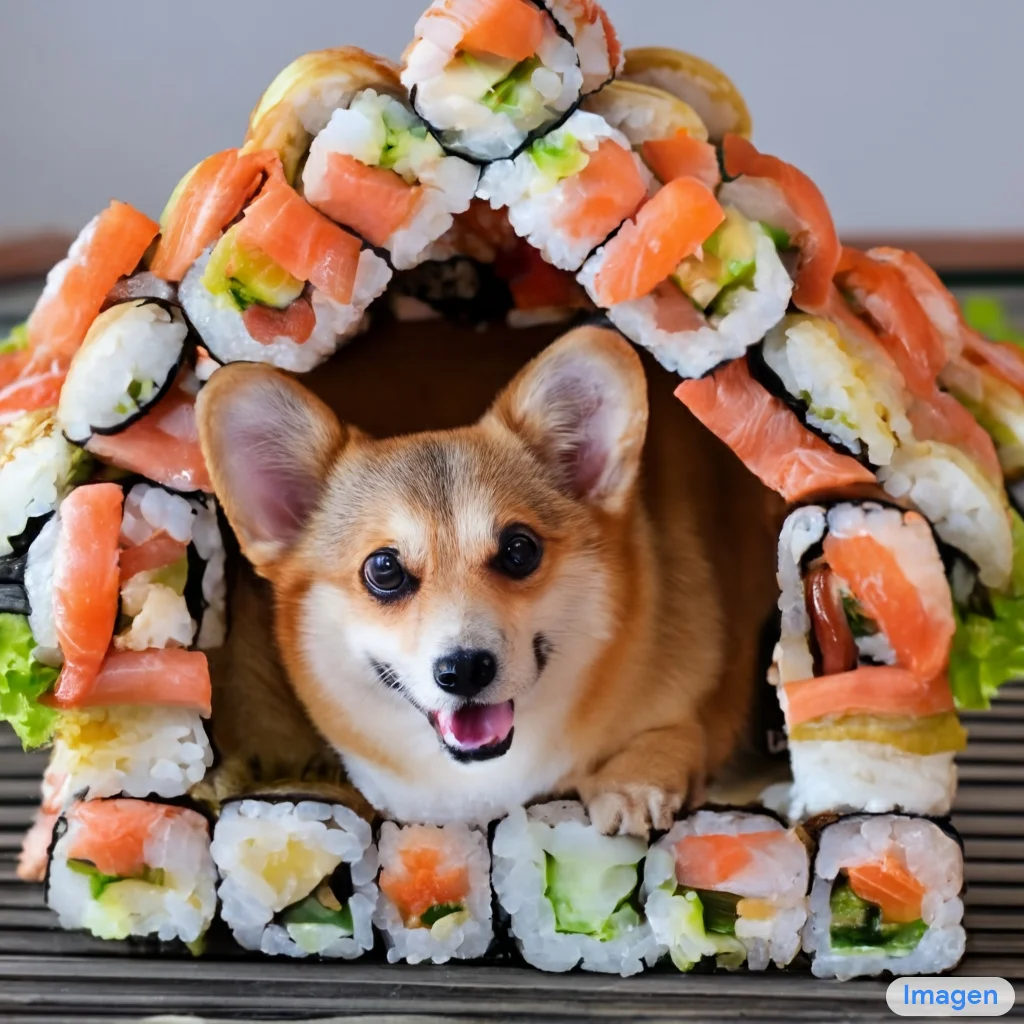
\includegraphics[width=7cm]{data/dog-in-sushihouse.png}
		\vfill
	\end{frame}

	\begin{frame}{Models} % Finn.no data
		\centering
		\vfill
		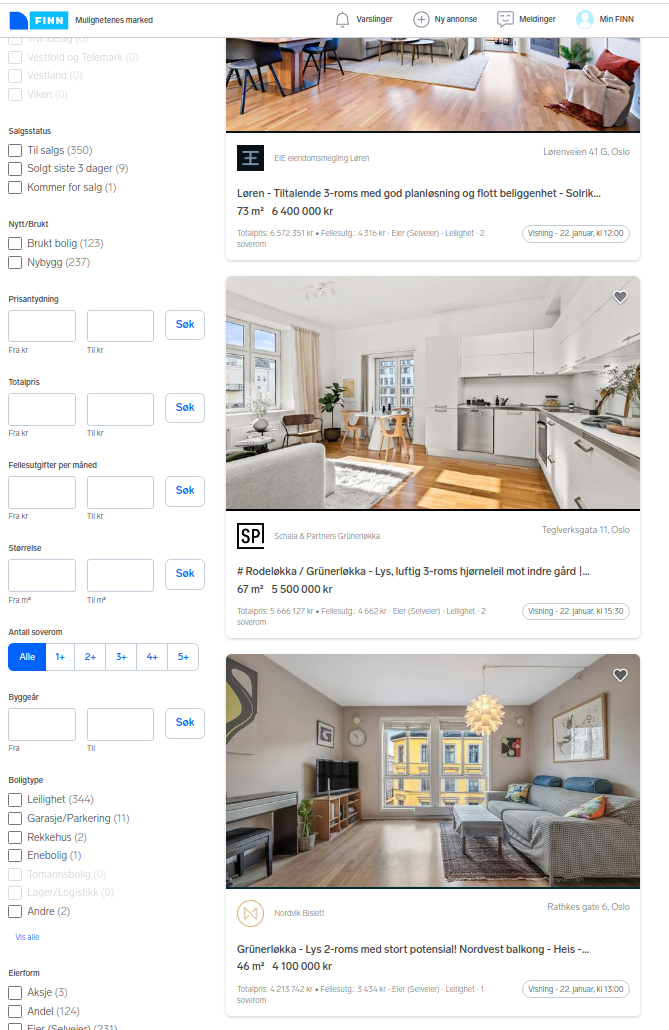
\includegraphics[height=7cm]{data/finn.png}
		\vfill
	\end{frame}

	\begin{frame}{Summary}
		\colorlet{answers}{cyan}
		\vfill
		\begin{itemize}
			\item{What is a statistical learning model?\\
				  \textcolor{answers}{A formula representing the relationship between inputs and outputs}}
			\item{What is a loss function?\\
				  \textcolor{answers}{A function quantifying how good a model is}}
			\item{How do we train a statistical learning model?\\
				  \textcolor{answers}{Gradual updates of parameters using gradient descent}}
			\item{How does a (deep) neural network work?\\
				  \textcolor{answers}{Sequentially applying (non-linear) artificial neurons to inputs}}
			\item{What operations does a convolutional neural network use?\\
				  \textcolor{answers}{Alternating convolutions and pooling}}
			\item{What is transfer learning?\\
				  \textcolor{answers}{Retraining an already trained model for a new problem}}
			\item{What is overfitting?\\
				  \textcolor{answers}{When a model learns patterns in the training data that does not hold generally}}
			\item{How do we combat it?\\
				  \textcolor{answers}{Rigorous testing, regularization and data augmentation}}
		\end{itemize}
		\vfill
	\end{frame}
\end{document}
